%!TEX root = ../Report.tex
\chapter{Requisitos e Arquitetura do Sistema}
\label{chp:requirements}
\section{Requisitos do Sistema}
Esta secção apresenta as especificações gerais dos requisitos do sistema. As seguintes subseções descrevem, em primeiro lugar, o processo de levantamento de requisitos e de seguida o contexto, os atores e os respetivos casos de uso. Por fim, são especificados os requisitos não funcionais do sistema, bem como as dependências do sistema e suposições.

\subsection{Levantamento de requisitos}
O levantamento de requisitos foi realizado na primeira fase de desenvolvimento do projeto,  na fase inicial de desenvolvimento. Foi realizada uma reunião com os Professore Flávio Meneses e o Professor Daniel Corujo na qual foram expostos os principais objetivos da plataforma.\newline
Desse modo, foram tomadas as seguintes decisões:
\begin{itemize}[noitemsep]
    \item Uma plataforma web será o foco principal do projeto sendo que a possibilidade de trabalhar com o nó móvel (também denominado de robô) foi movida para trabalho futuro devido ao facto do mesmo estar a ser alvo de reestruturações mecânicas e eletrónicas;
    \item A utilização da plataforma está restrita para utilizadores autenticados.
        \SubItem{Numa primeira fase serão criados, por um administrador do sistema, utilizadores próprios da plataforma (com um sistema de login com utilizador e palavra passe);}
        \SubItem{Numa fase posterior perspectiva-se a integração com as credenciais de colaboradores do IT através do LDAP.}
    \item Permitir a reconfiguração da rede de nós através da plataforma assim como a visualização dos dados de cada nó e os resultados das variadas experiências.
\end{itemize}

\subsection{Contexto}
Redes sem fios e, mais em particular redes móveis, têm sido um assunto bastante discutido nos dias que correm. Trabalhos de investigação e de inovação têm-se deparado com dificuldades na realização de testes ou experiências em ambiente real. Tal pode acontecer devido ao preço do material, condições ambientais ou difícil reprodução das condições ou ambientes sem fios. Para solucionar este problema surge a plataforma AMazING, uma plataforma de testes wireless com uma interface apelativa e fácil de utilizar.\newline\\
A plataforma foi desenvolvida de modo a facilitar a configuração dos nós necessários para cada experiência. O utilizador poderá agendar e realizar a sua experiência num ambiente o mais real possível.\newline
É importante referir que, a execução de vários testes em simultâneo seria possível desde que fossem utilizados nós distintos ou fosse garantido o isolamento, através de SDN, no switch. No entanto, devido à complexidade e aos conhecimentos de redes necessários para o desenvolvimento desta feature, foi considerado impossível a implementação da mesma no tempo disponível para a realização do projeto.\newline\\
Por este motivo, sempre que um utilizador pretenda agendar uma experiência, todos os nós ficam reservados para ele durante um determinado espaço de tempo. 
No menu principal está disposta a grelha de nós e as várias operações possíveis estão divididas em secções na barra de navegação, sendo que cada secção pode ter subsecções que permitem realizar funcionalidades mais específicas.


\subsection{Atores}
A desenvolvimento da interface gráfica foi levado a cabo tendo em conta que a plataforma será utilizada por pessoas que à partida são experientes na sua área, porém mantendo a interface simples de modo a ser de uso fácil. De seguida, enumeramos uma classificação dos atores que irão utilizar a plataforma:
\begin{itemize}[noitemsep]
    \item \textbf{Utilizador - Begginer}  – O João é estudante de Mestrado e está a realizar a sua tese no Instituto de Telecomunicações. Encontra-se num projeto de investigação que envolve testes de comunicação (com e sem fios) e desenvolvimento de novos protocolos de redes.\newline 
    O João precisa de realizar os seus testes num ambiente o mais real possível evitando simuladores virtuais. \newline
    O João é um utilizador iniciante, (nível 1) e só lhe é permitido utilizar os templates ao utilizar o sistema. e carregar ficheiros de execução para as APUs.
    \item \textbf{Utilizador - Advanced}  - O João recebe acesso de utilizador avançado (nível 2) o que lhe permite ter acesso direto ao terminal das APUs durante a realização de sua experiência. Podendo assim realizar a instalação de drivers, implementação de protocolos e outros serviços necessários para a realização da experiência
    \item \textbf{Administrador} - O Manuel é professor e Doutorado em Redes e Telecomunicações. É um dos responsáveis pelo Instituto de Telecomunicações e tem experiência em vários projetos relacionados com o desenvolvimento e implementação de novos protocolos de redes e telecomunicações.\newline
    O Manuel precisa de garantir o funcionamento e o acesso aos recursos disponibilizados no IT. 
\end{itemize}

\subsection{Casos de Uso}
Nas imagens seguintes, apresentamos os modelos de casos de uso(CaU) da solução. 
\subsubsection{Utilizador/Tester}
\begin{figure}[!ht]
    \centering
    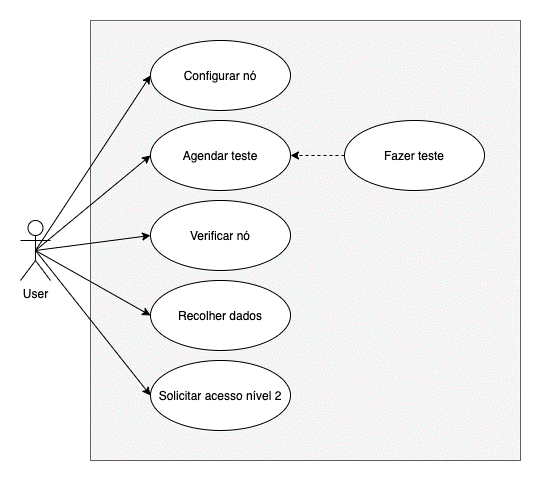
\includegraphics[height=0.36\textheight]{images/CaU1.png}
    \caption{Casos de uso do utilizador/Tester}
    \label{fig:cau1}
\end{figure}
Os casos de usos consoante a sua prioridade podem sintetizados de acordo com a seguinte tabela:
\begin{table}[ht]
    \centering
        \begin{tabular}{p{.25\textwidth}p{.50\textwidth}p{.15\textwidth}}
            \hline
            \textbf{CaU} &	\textbf{Descrição} &	\textbf{Prioridade} \\ 
            \hline
            Configurar Nó & Permite ao utilizador configurar um dado nó da rede como preferir. & Alta \\
            \hline
            Agendar/Fazer teste & Permite ao utilizador agendar a sua experiência e consequentemente efetuá-la no seu tempo alocado. & Alta \\
            \hline
            Verificar nó & Permite ao utilizador ver a informação de um nó (o seu estado, configuração, etc) & Alta \\
            \hline
            Recolher Dados & Permite ao utilizador recolher os dados provenientes da sua experiência. & Alta \\
            \hline
            Solicitar acesso de nível 2 & Permite que utilizador solicite a um administrador uma elevação dos seus privilégios na plataforma. & Alta \\
            \hline
        \end{tabular}
    \caption{Casos de uso do utilizador/Tester}
    \label{myTable}
\end{table}

\subsubsection{Administrador}
\begin{figure}[!ht]
    \centering
    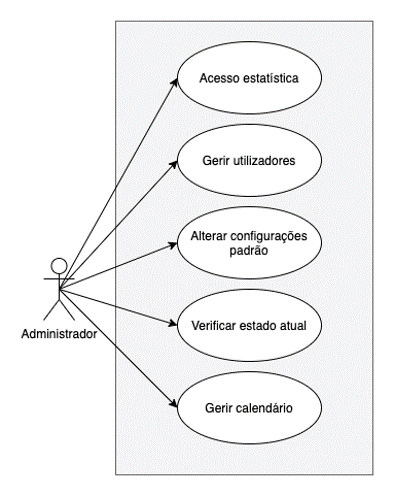
\includegraphics[height=0.4\textheight]{images/CaU2.png}
    \caption{Casos de uso do Administrador}
    \label{fig:cau2}
\end{figure}
Os casos de usos consoante a sua prioridade podem sintetizados de acordo com a seguinte tabela:
\begin{table}[ht]
    \centering
        \begin{tabular}{p{.25\textwidth}p{.50\textwidth}p{.15\textwidth}}
            \hline
            \textbf{CaU} &	\textbf{Descrição} &	\textbf{Prioridade} \\ 
            \hline
            Acesso a estatísticas & Permite ao administrador aceder às estatísticas da plataforma. & Alta \\
            \hline
            Gerir Utilizadores & Permite ao administrador gerir os utilizadores da plataforma assim como elevar o seu nível. & Alta \\
            \hline
            Adicionar/alterar Configurações padrões & Permite ao administrador adicionar/alterar configurações padrão dos nós & Alta \\
            \hline
            Verificar estado atual & Permite ao administrador verificar o estado atual da rede AMazING e dos seus nós. & Alta \\
            \hline
            Gerir Calendário & Permite ao administrador ver e gerir o calendário e os testes agendados. & Alta \\
            \hline
        \end{tabular}
    \caption{Casos de uso do Administrador}
    \label{myTable}
\end{table}

\newpage

\subsection{Requisitos não funcionais}
Abaixo, apresentamos os requisitos não funcionais do sistema.
\begin{itemize}
    \item \textbf{Usabilidade: } dado o principal propósito da aplicação, é necessário que esta seja simples de aprender e utilizar;
    \item \textbf{Autenticação:} A utilização da aplicação deve ser disponível apenas para utilizadores do IT 
        \SubItem{Numa primeira fase, adicionados ao sistema por um administrador;}
        \SubItem{Numa segunda fase, possuindo autenticação pelas credenciais de colaboradores do IT através do LDAP.}
    \item \textbf{Controlo:} O administrador do sistema deve ser capaz de configurar e realizar a manutenção do sistema;
    \item \textbf{Dados:} Os utilizadores do sistema deve conseguir aceder aos dados da experiência realizada.

\end{itemize}

\subsubsection{Suposições e Dependências}
Para o funcionamento completo do sistema, é necessário que sejam configurados os seguintes:
\begin{table}[ht]
    \centering
        \begin{tabular}{|p{.30\textwidth}|p{.60\textwidth}|}
            \hline
            \textbf{Hardware} &	\textbf{Software}\\ 
            \hline
            \begin{itemize}
                \item APUs
                \item Switch Aruba
            \end{itemize}
            & 
            \begin{itemize}
                \item Base de Dados Relacional de linguagem SQL
                \item Flask
                    \SubItem{No servidor principal}
                    \SubItem{Em cada uma das APUs}
                \item Django + SQLite
                \item Web SSH server
            \end{itemize}
            \\
        \hline
        \end{tabular}
    \caption{Componentes necessárias para o funcionamento}
    \label{myTable}
\end{table}

\section{Arquitetura do sistema}
Esta secção apresenta uma vista geral da arquitetura do sistema: os seus modelos de domínio, físico e tecnológico e a relação entre as componentes de cada um.
\subsection{Modelo Físico}
O modelo físico, representado na Figura 4, apresenta uma vista de alto nível da arquitetura física do sistema, as suas componentes, as suas interações e implementação. \newline\\
Do lado do utilizador, através de um navegador o utilizador vai aceder à plataforma que está hospedada no servidor utilizando protocolos HTTP.\newline\\
O servidor que está a hospedar a plataforma, este servidor seria uma VM localizada no IT, conecta-se então por LAN ao switch Aruba (componente descrito no capítulo 2), que por sua vez comunica com os nós presentes na rede de testes em causa, sendo que no nosso caso são as APUs que nos foram disponibilizadas.\hfill
\begin{figure}[!ht]
    \centering
    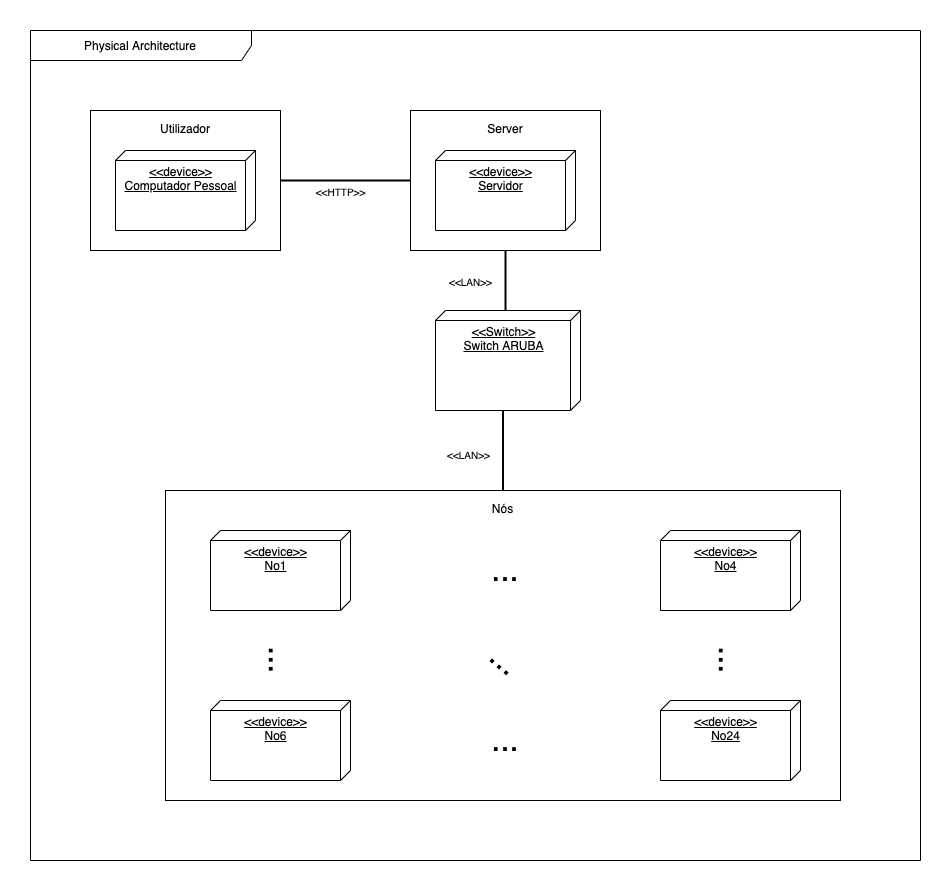
\includegraphics[height=0.63\textheight, width=1\textwidth]{images/physical_arch.png}
    \caption{Modelo Físico}
    \label{fig:fisico}
\end{figure}
É necessário que todas  as instâncias sejam acessíveis entre si, com exceção das bases de dados, onde, a Relacional só necessita estar acessível para o servidor principal Flask. O SQLite só necessita estar acessível para o servidor Django. É de realçar que o Switch Aruba teve que ser substituído devido aos impactos causados pelo Covid-19.

\subsection{Modelo Tecnológico}
O modelo tecnológico fornece uma vista sobre as tecnologias utilizadas pelo sistema. A figura seguinte demonstra como estas se relacionam entre si.

\begin{figure}[!ht]
    \centering
    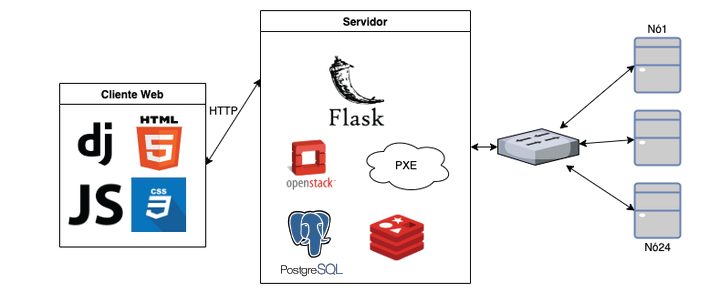
\includegraphics[height=0.3\textheight]{images/tecno.png}
    \caption{Modelo Tecnológico}
    \label{fig:tecno}
\end{figure}
\hfill\break
No lado do frontend, foi utilizada a framework Django que funciona sob a linguagem Python juntamente com HTML, JavaScript e CSS o que nos permitiu o desenvolvimento de uma plataforma web intuitiva e responsiva.\newline\\
No que toca ao armazenamento de dados, este é feito do lado do servidor e através do PostgreSQL - projeto open-source baseado em MySQL.\newline\\
Todas as ferramentas visíveis na imagem foram apresentadas e discutidas no capítulo 2. No que toca à sua implementação, razão de utilidade e a forma como interagem umas com as outras, no caso particular do projeto, serão discutidas abaixo.
\newpage
\hfill\break